\documentclass[11pt]{article}
\usepackage[margin=1in]{geometry}
\usepackage{amsmath,amssymb}
\usepackage{booktabs}
\usepackage{graphicx}
\usepackage[numbers,sort&compress]{natbib}
\usepackage{hyperref}
\usepackage{xcolor}
\usepackage{microtype}
\usepackage{algorithm}
\usepackage[noend]{algpseudocode}
\usepackage{listings}

\definecolor{codebg}{HTML}{F6F6F4}
\definecolor{codecomment}{HTML}{52514E}
\definecolor{codekw}{HTML}{1F5FAE}
\lstset{
  language=Python, basicstyle=\ttfamily\footnotesize, backgroundcolor=\color{codebg},
  keywordstyle=\color{codekw}\bfseries, commentstyle=\color{codecomment}\itshape,
  stringstyle=\color{codecomment}, showstringspaces=false, frame=single, rulecolor=\color{codebg},
  framesep=4pt, xleftmargin=6pt, xrightmargin=6pt, columns=fullflexible, keepspaces=true,
  breaklines=true, captionpos=b, upquote=true,
}

% Placeholder for numbers still to be filled in.
\newcommand{\TBD}[1]{\textcolor{red}{[TBD: #1]}}

\title{Monitoring Models Before the Labels Arrive:\\
A Benchmark for Performance Estimation, Drift Detection and Retraining\\
under Natural Drift and Label Delay}
\author{Raj Kumar Myakala\\ Independent Researcher\\}
\date{}

\begin{document}
\maketitle

\begin{abstract}
Deployed models are monitored long before their true labels arrive: a mortgage default is
known up to two years after the loan is made. Yet drift detectors and label-free performance
estimators are usually evaluated on artificially injected drift with labels available
immediately. We present an open benchmark that replays five real, timestamped data sources
(Freddie Mac mortgages, US Census ACS, CDC BRFSS, NYC taxi trips and TabReD) as streams in which a
monitor sees each label only when it would have arrived in practice, including the
\emph{natural} label delay of mortgage defaults. The benchmark scores four tasks on eight
experiments: estimating the performance of a new batch, estimating the performance of the
partly labeled ``in-flight'' book, detecting degradation, and deciding when to retrain,
the last scored as regret against a hindsight-optimal schedule. Three findings stand out.
(1) Input-drift tests (PSI, Kolmogorov--Smirnov, MMD, domain classifiers) alarm in every
period of the median experiment: on real data the inputs always change. (2) Label-free
estimators miss shocks that change outcomes but not inputs (the 2007--08 mortgage
crisis), while label-based monitoring sees them about two years late. (3) A fixed retraining
calendar beats monitor-triggered retraining in most experiments. We also propose
delay-adjusted CBPE, which uses early-arriving labels without being biased by them. It gives
the best degradation alarm overall (median rank correlation with true degradation 0.58,
precision 0.84). Its chain-ladder form fails, like actuarial chain-ladder methods, under
calendar-time shocks such as COVID forbearance; an age--period--cohort hazard variant fixes
this and gives the lowest in-flight error on Freddie Mac in three of four cases over five
seeds, e.g.\ 31\% lower default-rate error than the best label-based baseline across the
2007--2024 period. Code, data loaders and a leaderboard are released under the MIT license.
\end{abstract}

\section{Introduction}

Teams that run models in production ask two questions continually: \emph{is the model still
working}, and \emph{should we retrain it}? Answering with labels is often impossible in time.
A credit model's outcome (default within 24 months) is fully known only two years after each
decision; insurance conversions, medical outcomes and fraud chargebacks arrive weeks to months
late. Monitoring therefore relies on proxies: tests that the input distribution has shifted
\citep{rabanser2019failing,gretton2012kernel}, estimators that predict accuracy from the model's
own confidence \citep{garg2022atc,guillory2021doc,nannyml}, and streaming detectors on whatever
labels have arrived \citep{bifet2007adwin,gama2014survey}.

These methods are rarely evaluated under the conditions they are meant for. Benchmarks
typically inject synthetic drift into shuffled data and reveal each label immediately
\citep{cerqueira2026drift}; distribution-shift benchmarks with natural shift
\citep{koh2021wilds,yao2022wildtime} evaluate models, not monitors, and ignore when labels
arrive. Delayed labels have been studied for stream classifiers \citep{grzenda2020delayed}, but
not as the central obstacle to monitoring.

We build a benchmark around that obstacle. Our contributions:
\begin{enumerate}
  \item \textbf{Streams with label arrival times.} Five public sources replayed in time
  order; each row carries the time it is scored and the time its label becomes known. For
  Freddie Mac mortgages the arrival is natural: a default is known in the month it happens,
  a repayment only when the 24-month window closes (Section~\ref{sec:benchmark}).
  \item \textbf{Four tasks with leakage-free evaluation}: next-batch estimation, in-flight
  book estimation, degradation detection, and retraining decisions scored against a
  hindsight-optimal schedule computed by dynamic programming (Section~\ref{sec:tasks}).
  \item \textbf{Delay-adjusted CBPE}, a chain-ladder \citep{mack1993chainladder} correction that
  lets confidence-based estimation use early, biased labels, and an age--period--cohort hazard
  variant robust to calendar-time shocks (Section~\ref{sec:method}).
  \item \textbf{An empirical study} of 11 detectors, 8 estimators and 9 retraining policies on
  8 experiments (Section~\ref{sec:results}), with a public leaderboard.
\end{enumerate}

\section{Related work}

\paragraph{Drift detection.} Two-sample tests on inputs or model outputs
\citep{rabanser2019failing}, kernel tests \citep{gretton2012kernel}, domain classifiers, and
the population stability index used in credit risk flag that \emph{data} changed. Streaming
detectors such as ADWIN \citep{bifet2007adwin} monitor error rates and therefore need labels;
see \citet{gama2014survey} for a survey.

\paragraph{Label-free performance estimation.} ATC \citep{garg2022atc} and DoC
\citep{guillory2021doc} predict accuracy from confidence; CBPE \citep{nannyml} computes expected
confusion matrices from calibrated probabilities. All are exact under pure covariate shift with
calibration and fail under concept shift; label-shift estimators \citep{lipton2018bbse} assume
$P(x \mid y)$ is fixed. None uses the labels that do arrive early.

\paragraph{Benchmarks with natural shift.} Folktables \citep{ding2021folktables} exposes
year-to-year census shift; TabReD \citep{rubachev2024tabred} supplies industrial tabular data with
time-based splits; WILDS and Wild-Time \citep{koh2021wilds,yao2022wildtime} cover natural shift
for model robustness. Our benchmark reuses Folktables and TabReD data but evaluates monitors and
adds label arrival.

\paragraph{Delayed outcomes in actuarial science.} Insurers estimate claims incurred but not
yet reported with chain-ladder development patterns \citep{mack1993chainladder}; competing-risk
models \citep{fine1999competing} handle outcomes that can be pre-empted (a loan that repays cannot
default). Our method borrows both ideas.

\section{Benchmark}\label{sec:benchmark}

\paragraph{Stream format.} A stream is a table of prediction events. Row $i$ has features
$x_i$, an event time $t_i$ when the model scores it, an eventual label $y_i$ (possibly never
resolved) and a label time $\tau_i \ge t_i$ when $y_i$ becomes known. At any decision time
$s$, a monitor may use $y_i$ only if $\tau_i \le s$.

\paragraph{Data.} Table~\ref{tab:streams} lists the streams. Freddie Mac
\citep{freddiemac_sflld}: 1.36M loans originated 1999--2026 (the public 50k-per-year sample);
label: 90+ days delinquent or a credit-loss termination within 24 months of first payment; the
label time is the month of the event, or the month the loan reaches age 24 or prepays. Age is
counted in calendar months: the reported loan age is reset when a loan is modified, which would
otherwise let defaults years later count as early ones. ACS
\citep{ding2021folktables}: income above \$50k, 2014--2024 (2020 has no standard release),
relationship and state codes harmonized across years. BRFSS \citep{cdc_brfss}: diagnosed
diabetes, 2011--2024, ordered by interview month, 28 variables harmonized across renamings.
NYC taxi \citep{nyc_tlc}: card trips 2019--2021, label: tip $\ge$ 25\% of fare. TabReD
\citep{rubachev2024tabred}: the three binary tasks. Streams other than Freddie Mac receive a
simulated constant delay (Table~\ref{tab:streams}).

\begin{table}[t]
\centering
\caption{Experiments. Delay: natural, or simulated constant delay.}
\label{tab:streams}
\small
\begin{tabular}{llrlll}
\toprule
Experiment & Target & Rows & Delay & Trained on & Monitored \\
\midrule
freddie\_2007 & default $\le$24m & 1.36M & natural & 1999--2003 & 2007Q1--2024Q1 (q) \\
freddie\_2016 & default $\le$24m & 1.36M & natural & 2010--2012 & 2016Q1--2024Q1 (q) \\
acs\_income\_2016 & income $>$\$50k & 1.0M & 365 d & 2014 & 2016--2024 (y) \\
brfss\_2014 & diabetes & 1.68M & 180 d & 2011--mid 2013 & 2014--2025 (q) \\
tlc\_2019 & tip $\ge$25\% & 1.8M & 30 d & Feb--May 2019 & Jul 2019--Dec 2021 (m) \\
tabred\_homecredit & default & 382k & 90 d & Jan--May 2019 & 14 months (m) \\
tabred\_homesite & conversion & 261k & 30 d & Jan--Aug 2013 & 20 months (m) \\
tabred\_ecom & repeat purchase & 160k & 14 d & Mar 1--17 2013 & 5 weeks (w) \\
\bottomrule
\end{tabular}
\end{table}

\paragraph{Training without label leakage.} At the training date, a model may only learn from
cohorts whose labels have (at least 95\%) arrived. Using partly labeled cohorts is a common
silent error: early-arriving labels (defaults) are over-represented. The last 12 months of
trainable cohorts form the reference window on which monitors are calibrated. The model is a
gradient-boosted tree ensemble; it is then frozen.

\section{Tasks}\label{sec:tasks}

\paragraph{T1: next-batch estimation.} For each period, estimate the frozen model's metric
(AUC, positive rate, and accuracy where classes are balanced) on the batch scored in that
period, using its scores and the labels arrived by the period's end. Score: mean absolute error
(MAE) over periods, with 95\% moving-block bootstrap intervals over periods.

\paragraph{T2: in-flight book estimation.} For long-horizon labels, a new batch's outcome
depends on events that have not happened yet: Freddie Mac loans made in 2019Q1 defaulted at
4.4\% because of a pandemic a year later. The question a lender can answer is the state of its
\emph{book}: all loans scored in the last 24 months, part of which are already labeled.
Same score as T1.

\paragraph{T3: degradation detection.} A period is \emph{degraded} if its true metric is
worse than the reference by more than $\Delta$ (any change, for positive rate). Each detector
returns a drift score and an alarm. Scores: Spearman correlation of the drift score with the
true degradation; AUROC for several $\Delta$; precision and recall of the alarms.

\paragraph{T4: retrain or not.} After each period a policy may retrain on the labels arrived
so far. We precompute one candidate model per decision point and its loss (log loss) on every
later period, so any policy is evaluated by lookup. Cost $=$ total loss $+\ \lambda \times$
retrains. We report regret against the hindsight-optimal schedule, found by dynamic
programming over which model serves each period, for $\lambda = \rho \cdot g$, where $g$ is the
average gain of one retrain under ``always retrain'' and $\rho \in \{0, 0.25, 1, 4\}$.

\paragraph{Protocol.} All four tasks share one walk-forward loop (Algorithm~\ref{alg:protocol}).
Its only source of information about labels is the set $\mathcal{K}(s) = \{i : \tau_i \le s\}$, so
a monitor cannot see a label before it would have arrived. The true metric of a batch is computed
from labels the monitor never sees, and only for batches whose labels eventually resolve (at
least 90\%); later batches still receive estimates but are not scored. This is the real
``labels have not arrived'' frontier: for Freddie Mac it begins in 2024Q2.

\begin{algorithm}[t]
\caption{Walk-forward evaluation shared by all tasks}
\label{alg:protocol}
\begin{algorithmic}[1]
\Require stream $\{(x_i, y_i, t_i, \tau_i)\}$, training date $s_0$, period length (month/quarter/year)
\State $C \gets$ cohorts (periods) before $s_0$ whose labels are $\ge 95\%$ arrived by $s_0$
\State fit model $f$ on $C$ minus its last 12 months; reference window $R \gets$ last 12 months of $C$
\State calibrate each monitor $m$ on $\{(f(x_i), y_i) : i \in R\}$
\For{each period $P$ starting at or after $s_0$, in time order}
  \State $s \gets$ end of $P$; \quad $B \gets \{i : t_i \in P\}$; \quad $\mathcal{H} \gets \{i : t_i < \text{start of } P\}$
  \State history $\gets \{(f(x_i), t_i)\}_{i \in \mathcal{H}} \cup \{(y_i, \tau_i) : i \in \mathcal{H},\ \tau_i \le s\}$
  \State $\hat{v}_m \gets m(\{f(x_i), x_i\}_{i \in B}, \text{history})$ \Comment{estimate, drift score or alarm}
  \If{labels of $\ge 90\%$ of $B$ ever resolve}
    \State $v \gets$ metric of $f$ on $\{(f(x_i), y_i) : i \in B\}$ \Comment{hidden from every monitor}
    \State record $(P, m, \hat{v}_m, v)$
  \EndIf
\EndFor
\end{algorithmic}
\end{algorithm}

\section{Delay-adjusted CBPE}\label{sec:method}

CBPE treats calibrated scores $c_i$ as the probability each row is positive. Under concept
shift the calibration breaks; the labels that would reveal this arrive late, and the first to
arrive are biased: defaults arrive within months, repayments only after 24.

\paragraph{Arrival curves.} From mature rows (older than the longest observed delay) we
estimate $F(a)$, the probability that a positive's label has arrived by age $a$, and $G(a)$
for negatives.

\paragraph{Offset.} We model the true probability as $p_i = \sigma(\operatorname{logit} c_i +
\delta)$ and fit $\delta$ by maximum likelihood on the last 12 months of rows. Each row
contributes $p_i$ if its label arrived positive, $1-p_i$ if negative, and
\[ 1 - p_i F(a_i) - (1-p_i)\, G(a_i) \]
if still pending at age $a_i$. Early defaults therefore move $\delta$ at once without being
over-counted: a pending row is evidence of a negative only to the extent that a positive would
have arrived by now. With constant delay the method reduces to recalibrating on the most recent
complete labels.

\paragraph{Estimates.} For a new batch, the metric is computed as in CBPE from $p_i$ (expected
AUC from all positive--negative pairs; expected accuracy and positive rate in closed form). For
the in-flight book, arrived labels count as observed and pending rows use the posterior
$P(y_i = 1 \mid \text{pending}) = p_i(1-F(a_i)) / (1 - p_i F(a_i) - (1-p_i) G(a_i))$.
Algorithm~\ref{alg:dacbpe} summarizes the procedure.

\begin{algorithm}[t]
\caption{Delay-adjusted CBPE at decision time $s$}
\label{alg:dacbpe}
\begin{algorithmic}[1]
\Require calibrator $c(\cdot)$ fit on the reference window; history with arrived labels; batch scores
\State $D \gets$ longest observed delay $\tau_i - t_i$ among arrived labels
\State $M \gets$ rows with arrived labels and age $s - t_i \in [D, D + 36\text{ months})$ \Comment{mature rows}
\State $F, G \gets$ empirical CDFs of delays of positives / negatives in $M$
\State $W \gets$ rows of the last 12 months that are labeled or have $F(\text{age}) > 0.05$
\State $\hat\delta \gets \arg\max_\delta \sum_{i \in W} \log \ell_i(\delta)$, \quad $p_i(\delta) = \sigma(\operatorname{logit} c(f(x_i)) + \delta)$,
\Statex \hspace{\algorithmicindent} $\ell_i = p_i$ (arrived positive), $1 - p_i$ (arrived negative), $1 - p_i F(a_i) - (1 - p_i) G(a_i)$ (pending)
\State \textbf{new batch:} CBPE with $p_i(\hat\delta)$: positive rate $\frac{1}{n}\sum p_i$, expected AUC over pairs, expected accuracy
\State \textbf{in-flight book:} $q_i = y_i$ if arrived, else $p_i(1 - F(a_i)) / (1 - p_i F(a_i) - (1-p_i) G(a_i))$; metric from $q$
\end{algorithmic}
\end{algorithm}

\paragraph{Expected AUC.} Given probabilities $q_i$ that row $i$ is positive and scores $f_i$,
\[ \mathbb{E}[\mathrm{AUC}] \approx \frac{\sum_{i \ne j} q_i (1 - q_j) \left( \mathbb{1}[f_i > f_j] + \tfrac12 \mathbb{1}[f_i = f_j] \right)}
{\sum_i q_i \sum_j (1 - q_j) - \sum_i q_i (1 - q_i)}, \]
computed in $O(n \log n)$ by grouping equal scores and cumulating $1 - q$ over sorted scores (a
ratio-of-expectations approximation, exact as $n$ grows). A unit test checks it against Monte
Carlo draws of the labels.

\paragraph{Calendar-time shocks.} The development pattern $F$ is assumed stable. A shock that
hits rows of every age at once violates it: during COVID forbearance, loans of all ages became
90 days delinquent within months, which the method reads as the early edge of a much larger
wave and projects onto new loans. Actuarial chain-ladder methods share this weakness with
``calendar-year effects''.

\paragraph{Hazard variant.} We recast the method as an age--period--cohort model in discrete
time. On a monthly age grid, row $i$'s cumulative incidence without shocks is $p_i F(k)$, which
defines monthly hazard increments $L_i(k) = \log(1 - p_i F(k-1)) - \log(1 - p_i F(k))$.
\emph{Age} is fixed by $F$. \emph{Cohort}: $p_i = \sigma(\operatorname{logit} c_i + \delta_{g(i)})$
with one shift for the newest 12 months of rows and one for the 12 before. \emph{Period}: in
each of the last 24 calendar months $t$, every row alive gets the same extra hazard
$\lambda_t \ge 0$. With $S_i(k) = \exp(-\sum_{j \le k} [L_i(j) + \lambda_{t_i(j)}])$, a positive
arriving in month $k^*$ contributes $S_i(k^*-1) - S_i(k^*)$, a known negative $S_i(H)$, and a
pending row $S_i(a_i) - S_i(H)\,G(a_i)$. Older rows anchor $\lambda$: a calendar burst raises
their arrivals too, a new-cohort shift does not. This is what separates the two. Two design
choices matter. First, $\lambda_t \ge 0$: recent rows have no resolved negatives yet, so with
signed period effects ``nearly every row will be positive, just slowly'' fits as well as the
truth. Second, shocks are additive rather than proportional to each row's hazard, since
forbearance-type shocks hit safe and risky rows alike. New rows are projected with the newest
cohort's shift only; bursts are counted but not extrapolated. We fit by L-BFGS-B with analytic
gradients (Algorithm~\ref{alg:hazard}); Appendix~\ref{app:hazard} records the design choices that
the model needs to work, several of which we learned by failure.

\begin{algorithm}[t]
\caption{Hazard variant (DA-CBPE-HZ) at decision time $s$}
\label{alg:hazard}
\begin{algorithmic}[1]
\State $F, G \gets$ arrival curves as in Algorithm~\ref{alg:dacbpe}; $H \gets \lceil q_{0.995}(\text{positive delays}) \rceil$ months
\State $F \gets 0.99\,F + 0.01\,k/H$ on the monthly grid $k = 0..H$ \Comment{no month with zero arrival mass}
\State $W \gets$ informative rows of the last 24 months, minus pending rows past $H$; $g(i) \in \{\text{new}, \text{old}\}$ by cohort age $< 12$ months
\State for each row: calendar month $t_i(k)$ of every age month $k \le$ current age $a_i$ (the current partial month counted pro rata)
\State $\theta = (\delta_{\text{new}}, \delta_{\text{old}}, \lambda_1..\lambda_{24})$; \quad $p_i = \sigma(\operatorname{logit} c_i + \delta_{g(i)})$
\State $S_i(k) = \exp\!\big(-\sum_{j \le k} [\log\frac{1 - p_i F(j-1)}{1 - p_i F(j)} + \lambda_{t_i(j)}]\big)$
\State $\hat\theta \gets \arg\min_\theta -\sum_{i \in W} \log \ell_i(\theta) + \sum_t \lambda_t^2$ \ s.t.\ $\lambda_t \ge 0$ \Comment{L-BFGS-B, analytic gradient, warm start}
\Statex \hspace{\algorithmicindent} $\ell_i = S_i(k^*_i - 1) - S_i(\min(k^*_i, a_i))$ (positive), $S_i(H)$ (negative), $S_i(a_i) - S_i(H)\,G(a_i)$ (pending)
\State \textbf{new batch:} CBPE with $p_i(\hat\delta_{\text{new}})$ \Comment{bursts not projected forward}
\State \textbf{in-flight book:} arrived labels as observed; pending rows $q_i = \frac{S_i(a_i) - S_i(H)}{S_i(a_i) - S_i(H)\,G(a_i)}$ with fitted $\lambda$
\end{algorithmic}
\end{algorithm}

\section{Results}\label{sec:results}

\paragraph{Detection (T3).} Table~\ref{tab:detection} summarizes 16 cases (8 experiments $\times$
2 event types). Every input-drift test alarms in every period of the median case: lender
churn, interest-rate levels, a discontinued channel code and a field introduced in 2017 all
shift Freddie Mac's inputs without necessarily hurting the model. Their scores still rank
severity moderately (median $\rho$ 0.37--0.49), but their thresholds are unusable. The
delay-adjusted alarm both ranks degradation best (median $\rho$ 0.58) and alarms selectively
(32\% of periods, precision 0.84). ADWIN on arriving errors, the classic streaming setup, ranks
last: under delay it sees too little, too late. Figure~\ref{fig:detection} shows the trade-off;
per-experiment correlations and alarm statistics are in Appendix~\ref{app:results}
(Tables~\ref{tab:det-spearman} and~\ref{tab:det-alarms}).

\begin{figure}[t]
\centering
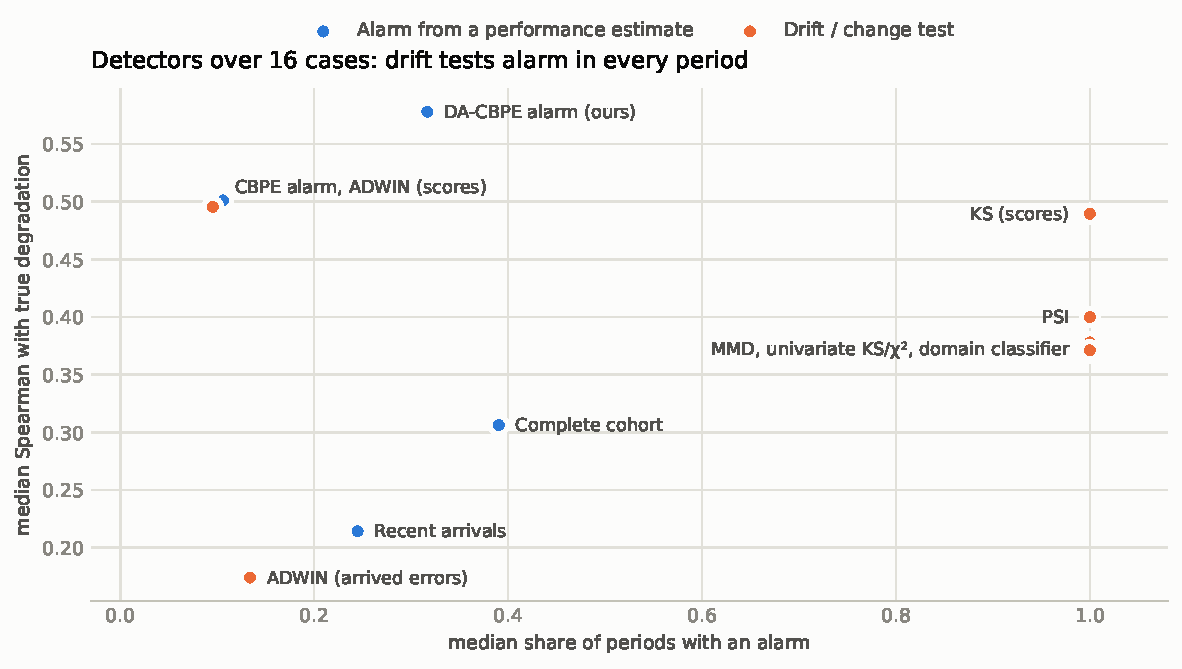
\includegraphics[width=0.85\linewidth]{../figures/detection_overview.pdf}
\caption{Each detector's median alarm rate against its median rank correlation with true
degradation, over 16 cases. Every input-drift test sits at an alarm rate of 1.0.}
\label{fig:detection}
\end{figure}

\begin{table}[t]
\centering
\caption{Degradation detection: medians over 16 cases.}
\label{tab:detection}
\small
\begin{tabular}{lrrrr}
\toprule
Detector & Spearman $\rho$ & Alarm rate & Precision & Recall \\
\midrule
Delay-adjusted CBPE alarm (ours) & \textbf{0.58} & 0.32 & \textbf{0.84} & 0.52 \\
CBPE alarm & 0.50 & 0.11 & 0.82 & 0.11 \\
ADWIN on scores & 0.50 & 0.10 & 0.67 & 0.13 \\
KS on scores & 0.49 & 1.00 & 0.48 & 1.00 \\
PSI & 0.40 & 1.00 & 0.44 & 1.00 \\
MMD & 0.38 & 1.00 & 0.52 & 1.00 \\
Univariate KS / $\chi^2$ & 0.37 & 1.00 & 0.48 & 1.00 \\
Domain classifier & 0.37 & 1.00 & 0.52 & 1.00 \\
Latest complete cohort alarm & 0.31 & 0.39 & 0.71 & 0.71 \\
Recent arrivals alarm & 0.21 & 0.24 & 0.63 & 0.40 \\
ADWIN on arrived errors & 0.17 & 0.13 & 0.83 & 0.19 \\
\bottomrule
\end{tabular}
\end{table}

\paragraph{Estimation (T1, T2).} Tables~\ref{tab:estimation} and~\ref{tab:inflight} report MAE over
five seeds. Seed-to-seed variation is small relative to the gaps between methods.

\emph{Next batch.} No method dominates. Label-free and delay-adjusted estimators are most
accurate when shift is mostly in the inputs (TabReD homesite and homecredit, BRFSS). With short
delays and a drifting label, simply using the latest complete labels wins (ACS income under wage
inflation, NYC taxi tips, TabReD ecom). On short-horizon streams the hazard variant's extra
parameters are poorly anchored and cost accuracy (NYC taxi positive rate: 0.030 vs.\ 0.012 for the
chain-ladder form), so it should be preferred only where labels arrive over a long horizon. On
Freddie Mac the task is close to unanswerable: loans made in 2019Q1 defaulted at 4.4\% because of
a pandemic a year later.

\emph{In-flight book.} Here early labels pay off (Table~\ref{tab:inflight}). The hazard variant
has the lowest error in three of four cases. On freddie\_2007 its default-rate error is 0.0060
against 0.0087 for the best label-based baseline, and its AUC error 0.0180 against 0.0215;
block-bootstrap intervals of the paired differences exclude zero (default rate: $-0.0034$
[$-0.0076$, $-0.0004$] vs.\ waiting for complete cohorts; AUC: $-0.0058$ [$-0.0126$, $-0.0001$]
vs.\ labels to date). The exception is freddie\_2016 AUC, where labels to date is better (0.0263
vs.\ 0.0287; interval includes zero). All paired comparisons are in Table~\ref{tab:inflight-ci};
the accuracy-only estimators ATC and DoC are compared in Table~\ref{tab:accuracy}.

Figure~\ref{fig:freddie} shows the mechanism. CBPE stays near the reference default rate through
the 2007--08 crisis (loans made in 2008Q1: true 6.6\%, CBPE 1.0\%). Waiting for complete cohorts
sees the crisis about two years late and then reports it after it has passed (4.7\% for 2010Q1
loans against a true 0.6\%). On the in-flight book both delay-adjusted estimators react within
quarters. Under COVID, the chain-ladder form reads forbearance as the start of a much larger wave
(peak in-flight estimate 8.3\% against a true peak of 4.3\%); the hazard variant attributes it to
calendar months and peaks at 4.3\%.

\begin{table}[t]
\centering
\caption{Next-batch estimation. MAE, mean (std) over 5 seeds; lower is better, best in bold.}
\label{tab:estimation}
\scriptsize
\setlength{\tabcolsep}{3pt}
\resizebox{\textwidth}{!}{%
\begin{tabular}{llrrrrrr}
\toprule
Experiment & Metric & Ref. & Recent & Complete & CBPE & DA-CBPE & DA-CBPE-HZ \\
\midrule
acs\_income\_2016 & accuracy & 0.0369 (0.0018) & -- & \textbf{0.0087 (0.0002)} & 0.0314 (0.0024) & 0.0145 (0.0020) & 0.0154 (0.0021) \\
acs\_income\_2016 & pos. rate & 0.0929 (0.0015) & -- & 0.0199 (0.0002) & 0.0778 (0.0022) & \textbf{0.0178 (0.0006)} & 0.0202 (0.0014) \\
acs\_income\_2016 & AUC & 0.0096 (0.0020) & -- & \textbf{0.0019 (0.0003)} & 0.0071 (0.0021) & 0.0091 (0.0022) & 0.0090 (0.0022) \\
brfss\_2014 & pos. rate & 0.0093 (0.0009) & 0.0045 (0.0002) & 0.0052 (0.0002) & 0.0041 (0.0010) & \textbf{0.0033 (0.0004)} & 0.0039 (0.0006) \\
brfss\_2014 & AUC & 0.0106 (0.0007) & \textbf{0.0042 (0.0003)} & 0.0062 (0.0003) & 0.0050 (0.0001) & 0.0051 (0.0001) & 0.0051 (0.0001) \\
freddie\_2007 & pos. rate & \textbf{0.0108 (0.0000)} & 0.0140 (0.0000) & 0.0166 (0.0000) & 0.0123 (0.0003) & 0.0143 (0.0002) & 0.0122 (0.0009) \\
freddie\_2007 & AUC & 0.0498 (0.0034) & 0.0502 (0.0033) & 0.0471 (0.0025) & 0.0382 (0.0075) & \textbf{0.0360 (0.0063)} & 0.0375 (0.0069) \\
freddie\_2016 & pos. rate & \textbf{0.0140 (0.0000)} & 0.0166 (0.0000) & 0.0174 (0.0000) & 0.0140 (0.0004) & 0.0218 (0.0010) & 0.0142 (0.0011) \\
freddie\_2016 & AUC & 0.1054 (0.0063) & 0.0724 (0.0077) & \textbf{0.0422 (0.0029)} & 0.0726 (0.0044) & 0.0691 (0.0038) & 0.0713 (0.0039) \\
tabred\_ecom & pos. rate & \textbf{0.0697 (0.0019)} & 0.0772 (0.0000) & 0.0966 (0.0000) & 0.1741 (0.0094) & 0.1449 (0.0075) & 0.1717 (0.0213) \\
tabred\_ecom & AUC & 0.2316 (0.0255) & 0.1014 (0.0128) & \textbf{0.0717 (0.0154)} & 0.1133 (0.0288) & 0.1089 (0.0294) & 0.1083 (0.0292) \\
tabred\_homecredit & pos. rate & 0.0094 (0.0000) & 0.0119 (0.0000) & 0.0099 (0.0000) & 0.0089 (0.0019) & 0.0089 (0.0006) & \textbf{0.0086 (0.0005)} \\
tabred\_homecredit & AUC & 0.0180 (0.0027) & 0.0254 (0.0026) & 0.0185 (0.0034) & 0.0159 (0.0018) & \textbf{0.0159 (0.0017)} & 0.0159 (0.0017) \\
tabred\_homesite & pos. rate & 0.0236 (0.0016) & 0.0160 (0.0000) & 0.0160 (0.0000) & 0.0052 (0.0013) & \textbf{0.0046 (0.0015)} & 0.0051 (0.0017) \\
tabred\_homesite & AUC & 0.0137 (0.0017) & 0.0058 (0.0001) & 0.0056 (0.0003) & 0.0051 (0.0020) & \textbf{0.0048 (0.0020)} & 0.0049 (0.0021) \\
tlc\_2019 & accuracy & 0.0062 (0.0005) & 0.0036 (0.0001) & \textbf{0.0031 (0.0000)} & 0.0055 (0.0004) & 0.0086 (0.0003) & 0.0144 (0.0005) \\
tlc\_2019 & pos. rate & 0.0339 (0.0013) & 0.0085 (0.0000) & \textbf{0.0078 (0.0000)} & 0.0164 (0.0010) & 0.0116 (0.0002) & 0.0301 (0.0007) \\
tlc\_2019 & AUC & 0.0189 (0.0009) & 0.0060 (0.0002) & \textbf{0.0052 (0.0001)} & 0.0057 (0.0002) & 0.0078 (0.0003) & 0.0073 (0.0001) \\
\bottomrule
\end{tabular}}
\end{table}

\begin{table}[t]
\centering
\caption{In-flight book estimation (Freddie Mac, natural label delay). MAE, mean (std) over 5 seeds; lower is better, best in bold.}
\label{tab:inflight}
\scriptsize
\setlength{\tabcolsep}{3pt}
\resizebox{\textwidth}{!}{%
\begin{tabular}{llrrrrrr}
\toprule
Experiment & Metric & Ref. & To date & Complete & CBPE & DA-CBPE & DA-CBPE-HZ \\
\midrule
freddie\_2007 & pos. rate & 0.0102 (0.0000) & 0.0090 (0.0000) & 0.0087 (0.0000) & 0.0119 (0.0003) & 0.0065 (0.0000) & \textbf{0.0060 (0.0008)} \\
freddie\_2007 & AUC & 0.0462 (0.0035) & 0.0215 (0.0009) & 0.0394 (0.0016) & 0.0333 (0.0086) & 0.0220 (0.0046) & \textbf{0.0180 (0.0021)} \\
freddie\_2016 & pos. rate & 0.0124 (0.0000) & 0.0088 (0.0000) & 0.0083 (0.0000) & 0.0127 (0.0002) & 0.0103 (0.0001) & \textbf{0.0060 (0.0003)} \\
freddie\_2016 & AUC & 0.0968 (0.0058) & \textbf{0.0263 (0.0012)} & 0.0355 (0.0018) & 0.0692 (0.0037) & 0.0422 (0.0023) & 0.0287 (0.0024) \\
\bottomrule
\end{tabular}}
\end{table}


\begin{figure}[t]
\centering
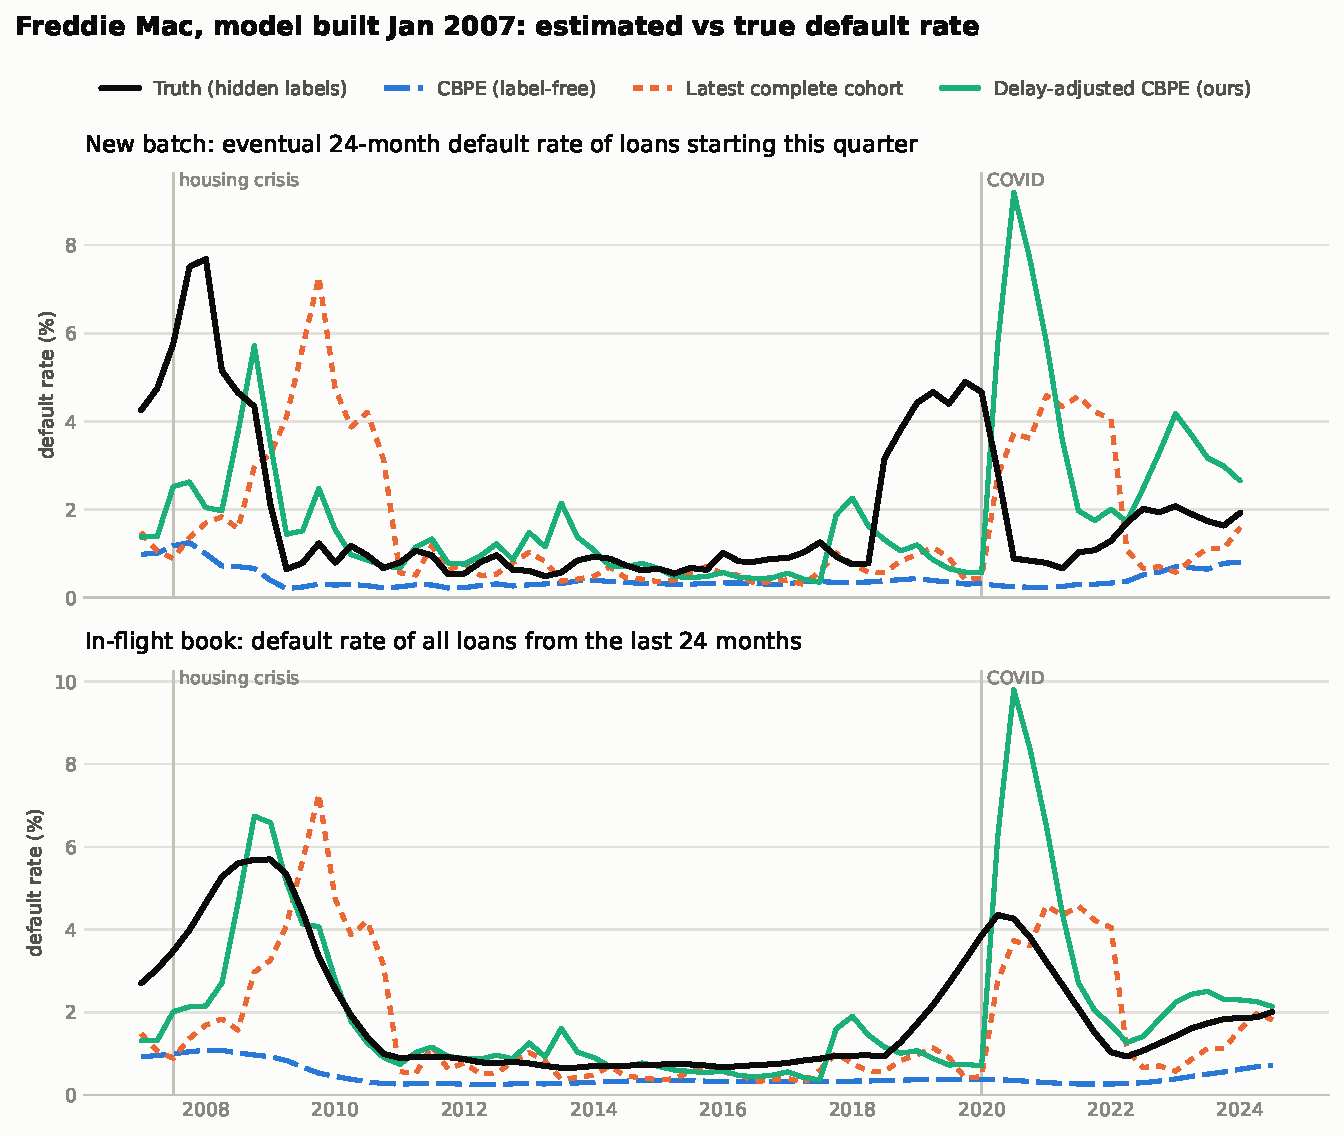
\includegraphics[width=\linewidth]{../figures/freddie_2007_default_rate.pdf}
\caption{Freddie Mac, model built January 2007. Top: eventual default rate of each quarter's
new loans. Bottom: default rate of the in-flight book (loans from the last 24 months).}
\label{fig:freddie}
\end{figure}

\paragraph{Synthetic checks.} Two controlled streams isolate the two kinds of shock: a lasting
shift (the outcome rate of new cohorts jumps) and a calendar burst (for four months every active
loan has an extra 3\% monthly default hazard, new cohorts unaffected). The chain-ladder form tracks
the lasting shift best (in-flight MAE 0.007 vs.\ 0.050 for complete cohorts) but its error grows
more than tenfold under the burst (0.094). The hazard variant gives up a little on the lasting
shift (0.010) and cuts the burst error to 0.030, the best of all methods.

\paragraph{Retraining (T4).} At moderate retraining cost ($\rho=1$) a fixed calendar is the best
policy in 5 of 8 experiments (with the period chosen in hindsight, which flatters it). Monitoring
helps on Freddie Mac: retraining on alarms from recently arrived labels wins on freddie\_2007, and
on CBPE alarms on freddie\_2016. Retraining on input-drift alarms is equivalent to always
retraining, since those tests always fire: cheapest when retraining is free, among the worst once
it costs anything. On tabred\_ecom retraining never pays: newer models train on too little data.
Full regret tables are in Appendix~\ref{app:results} (Table~\ref{tab:retrain}).

\section{Software}\label{sec:software}

The benchmark is a Python package, \texttt{lfmm}, released under the MIT license with all
experiment scripts.\footnote{\url{https://github.com/rajkumar160798/label-free-model-monitoring}}
It has four parts: downloaders that record every source file's URL and SHA-256 checksum; stream
loaders that build the label and its arrival time from the raw files; the four tasks; and the
methods, each a small class with \texttt{fit} on the reference window and one method that
answers the task. Listing~\ref{lst:estimate} runs the estimation task on any stream; adding a
method means subclassing \texttt{Estimator}, \texttt{Detector} or \texttt{Policy}
(Appendix~\ref{app:code}). Every listing in this paper is a runnable file in the repository's
\texttt{paper/snippets/} folder.

\begin{lstlisting}[caption={Estimating performance on a stream with delayed labels.}, label={lst:estimate}]
from lfmm.estimators import CBPE, DelayAdjustedCBPE, LatestCompleteCohort
from lfmm.harness import run_estimation

# Train on fully labeled cohorts before 2023, freeze, walk forward monthly.
result = run_estimation(
    stream, train_end="2023-01-01", freq="M", metrics=("roc_auc", "prevalence"),
    estimators=[CBPE(), DelayAdjustedCBPE(), LatestCompleteCohort(freq="M")],
)
print(result.summary())                     # MAE and bias per estimator
print(result.bootstrap_mae("prevalence"))   # 95% block-bootstrap intervals
print(result.compare("prevalence", "da_cbpe", "cbpe"))
\end{lstlisting}

Everything runs on a 16-core desktop without a GPU. Single task runs take from under a minute to
under half an hour per experiment (Appendix~\ref{app:impl}); the hazard estimator and the
domain-classifier and MMD detectors dominate the time.

\section{Limitations}

Simulated delays on six of eight experiments are constant; only Freddie Mac has natural arrival.
Estimation results cover five seeds (model randomness and, for sampled streams, the sample);
detection and retraining results are single runs with period-level summaries. The
fixed-calendar policy's period is chosen in hindsight. Regression tasks (five TabReD datasets)
are not yet supported. Freddie Mac and TabReD data cannot be redistributed; the benchmark ships
loaders and checksums, not data.

\section{Conclusion}

Monitoring benchmarks should model when labels arrive. Doing so shows that input-drift alarms
are uninformative on real data, that label-free and label-based estimators fail in opposite
directions, and that early-arriving labels, once their bias is corrected, close much of the gap.

\bibliographystyle{plainnat}
\bibliography{references}

\clearpage
\appendix

\section{Using the benchmark}\label{app:code}

Every listing below is a file in \texttt{paper/snippets/} and runs as shown against the released
package (it uses a small synthetic stream so it runs in seconds without downloading data).

\lstinputlisting[caption={Building a stream from any table of scored events
(\texttt{s1\_stream.py}).}, label={lst:stream}]{snippets/s1_stream.py}

\lstinputlisting[caption={Adding an estimator: implement \texttt{estimate}, which sees the batch's
scores and a \texttt{History} holding only labels that have arrived (\texttt{s3\_custom.py}).},
label={lst:custom}]{snippets/s3_custom.py}

\lstinputlisting[caption={Detection against an event definition, and the retrain-or-not task with
fixed and alarm-triggered policies (\texttt{s4\_detect\_retrain.py}).},
label={lst:detect}]{snippets/s4_detect_retrain.py}

{\sloppy
\paragraph{Running the paper's experiments.} The eight experiments are declared in
\texttt{lfmm.experiments.EXPERIMENTS} (stream loader, training date, period length, metrics and
event definitions). Each task has a script: \texttt{run\_estimation.py}, \texttt{run\_inflight.py},
\texttt{run\_detection.py}, \texttt{run\_retrain.py} and \texttt{run\_seeds.py}; tables and figures
are regenerated from their CSV outputs by \texttt{make\_tables.py}, \texttt{make\_appendix.py} and
\texttt{make\_figures.py}. Raw data are fetched by \texttt{python -m lfmm.download}, which writes a
manifest with the source URL and SHA-256 of every file; Freddie Mac and TabReD files, which need an
account or accepted terms, are downloaded by hand and registered with the same command.\par}

\section{Dataset construction}\label{app:data}

\begin{table}[h]
\centering
\caption{Streams after construction. Rows are those used in the experiments (ACS and BRFSS are
sampled per year from the full tables; NYC taxi keeps 50k card trips per month).}
\label{tab:data}
\scriptsize
\resizebox{\textwidth}{!}{%
\begin{tabular}{lllrrrll}
\toprule
Stream & Source & Years & Rows used & Num. & Cat. & Target & Positive rate \\
\midrule
Freddie Mac & SFLLD sample & 1999--2026 & 1,362,496 & 10 & 12 & default within 24 months & 0.4\%--4.8\% by year \\
ACS income & Census PUMS & 2014--2024 & 1.0M (of 16.6M) & 5 & 6 & income $>$ \$50k & 31.7\%--49.1\% \\
BRFSS & CDC survey & 2011--2024 & 1.68M (of 6.3M) & 8 & 17 & diagnosed diabetes & 12.4\%--14.6\% \\
NYC taxi & TLC trip records & 2019--2021 & 1.8M (of 140M) & 13 & 4 & tip $\ge$ 25\% of fare & 54.8\%--61.9\% \\
TabReD homecredit & TabReD & 2019--2020 & 381,664 & 612 & 82+2 bin. & loan default & 3.2\% \\
TabReD homesite & TabReD & 2013--2015 & 260,753 & 253 & 23+23 bin. & quote conversion & 18.8\% \\
TabReD ecom & TabReD & 2013 & 160,057 & 113 & 6 bin. & repeat purchase & 27.1\% \\
\bottomrule
\end{tabular}}
\end{table}

\paragraph{Freddie Mac.} Origination features: credit score, mortgage-insurance percentage, number
of units, combined and plain loan-to-value, debt-to-income, original balance, interest rate, term
and number of borrowers (numeric); first-time buyer, occupancy, channel, state, property type,
loan purpose, seller, super-conforming, program, relief refinance, valuation method and
interest-only flags (categorical). Sentinel codes (e.g.\ 9999 for credit score, 999 for ratios) are
set to missing. Identifiers, maturity date, MSA and postal code are dropped, and so is MI
cancellation, which is observed after origination and would leak. The number-of-borrowers field
changed coding in 2018Q2 (``2 or more'' became exact counts) and is capped at 2. The event is
delinquency of 90 days or more, REO acquisition, or a zero-balance code for third-party sale,
short sale, REO disposition or whole-loan sale, within 24 calendar months of the first payment.
A negative is known at month 24 or at an earlier prepayment (zero-balance code 01); loans with
neither never resolve. Four seller-owned modified loans whose first-payment date was reset years
after origination are dropped. Counting the window by the reported loan age instead of calendar
months would be wrong: Freddie Mac resets loan age at modification, which in a first version of
this benchmark turned 17.7\% of positives into defaults that happened years later.

\paragraph{ACS.} The Folktables ACSIncome task \citep{ding2021folktables}: employed adults (age
$> 16$, income $> \$100$, hours $> 0$, weight $\ge 1$), features age, education, hours, occupation,
place of birth (numeric) and class of worker, marital status, relationship, sex, race and state
(categorical). From 2019 the relationship field RELP was replaced by RELSHIPP with new codes; we map
RELSHIPP to RELP. The state column is ST until 2022 and STATE from 2023. Occupation codes switched to
the 2018 SOC scheme in 2018 and are left as they are, as a production pipeline would see them.
Income is nominal, so the positive rate rises with wages.

\paragraph{BRFSS.} Interviews are ordered by interview month (a survey year's last interviews fall
in the next calendar year). Variables renamed across years are merged (diabetes, sex, income,
kidney disease, depression, arthritis, cost barrier, personal doctor, race). From 2021 the income
variable splits the top band (\$50k+) into three; we cap it back to five bands. Employment is not
asked in 2011--2012 and health insurance is not asked of all ages in 2021--2022; those values stay
missing. Positive: ever told diabetes (excluding pregnancy-only); ``don't know'' and refusals are
dropped.

\paragraph{NYC taxi.} Credit-card trips only (cash tips are not recorded) with positive fare and
distance, duration 1--180 minutes, and pickup and drop-off within the file's month. Features:
passengers, distance, fare, surcharges and tolls, duration, hour, weekday, pickup and drop-off
zone, vendor, rate code and store-and-forward flag. The total amount is excluded because it
includes the tip; the airport fee exists only from 2021. The positive rate jumps from 25\% in
January 2019 to 58\% from February, coinciding with the congestion surcharge introduced on
1~February~2019 (we have not confirmed the cause), so the training window starts in February.

\paragraph{TabReD.} The authors' preprocessed arrays \citep{rubachev2024tabred}; rows ordered by the
timestamp in the first metadata column, which is in microseconds for homesite and in days for
homecredit and ecom. TabReD's own splits are not used: the walk-forward protocol replaces them.

\section{Implementation details}\label{app:impl}

\paragraph{Model.} Scikit-learn's histogram gradient boosting (300 iterations, learning rate 0.08,
early stopping on 10\% of the training rows, native categorical handling; categoricals with more
than 250 levels become integer codes). Features that are missing or constant in the training rows
are dropped. At most 500k training rows (300k for the retraining bank).

\paragraph{Protocol.} Trainable cohorts need $\ge 95\%$ of labels arrived; reference window = the last
12 months of trainable cohorts (a random 30\% when that would leave too little training data); truth
requires $\ge 90\%$ of a batch's labels to resolve. Retraining uses the last 60 months of trainable
cohorts.

\paragraph{Estimators.} Recent arrivals: labels arrived in the last 90 days ($\ge 200$ rows). Latest
complete cohort: newest monthly cohort with $\ge 95\%$ of labels arrived. CBPE: isotonic calibration
on the reference window. ATC and DoC: as published, with confidence $\max(p, 1-p)$. DA-CBPE: 12-month
fitting window, 36 months of mature rows for the arrival curves, up to 50k rows. Hazard variant:
24-month window, cohort split at 12 months, 24 calendar months, ridge 1, up to 20k rows,
$\lambda_t \in [0, 0.5]$, $\delta \in [-5, 5]$.

\paragraph{Detectors.} Univariate: KS (numeric) and $\chi^2$ (categorical) with Bonferroni correction,
scored by the largest effect size. PSI: 10 reference-quantile bins plus a missing bin, alarm at 0.25.
KS on scores: alarm at $p < 0.05$. Domain classifier: gradient boosting (100 iterations) on up to 5k
reference and 5k batch rows, 3-fold cross-validated AUC, alarm at 0.6. MMD: RBF kernel with median
bandwidth on standardized numeric features and the score, 1k rows per side, 100 permutations, alarm at
$p < 0.05$. ADWIN: $\delta = 0.002$, up to 2k values per batch. Estimator alarms fire when the estimate
is worse than the reference by more than the experiment's alarm $\Delta$: AUC 0.05 and default rate
0.01 for Freddie Mac; accuracy 0.03 and positive rate 0.05 for ACS; AUC 0.02 and positive rate 0.01
for TabReD homecredit; AUC 0.02 and positive rate 0.02 for the others.

\paragraph{Statistics.} Moving-block bootstrap over periods, block length 4, 2000 resamples; paired
comparisons resample the per-period difference. Estimation is repeated over 5 seeds (model
randomness, training subsample, and for ACS and BRFSS the per-year sample).

\paragraph{Compute.} One 16-core Windows desktop, no GPU. Measured times: next-batch estimation
under a minute per experiment without the hazard estimator; one hazard fit 3--11 seconds per
Freddie Mac quarter; detection on both Freddie Mac experiments about 20 minutes; the retraining bank
for freddie\_2016 about 8 minutes (33 models).

\section{Designing the hazard variant}\label{app:hazard}

The hazard variant took several attempts; each failure is instructive for anyone extending it.
Table~\ref{tab:ablation} lists every version we tried on the two synthetic streams of
Section~\ref{sec:results}, in the order we tried them.

\begin{table}[h]
\centering
\caption{Design ablation on synthetic data (MAE of the positive rate). Each row adds one change to
the previous one. The burst stream needs the calendar effect; the lasting-shift stream checks that
fixing it does not break what already worked.}
\label{tab:ablation}
\small
\resizebox{\textwidth}{!}{%
\begin{tabular}{lrrrr}
\toprule
& \multicolumn{2}{c}{Calendar burst} & \multicolumn{2}{c}{Lasting shift} \\
Version & next batch & in-flight & next batch & in-flight \\
\midrule
Chain-ladder DA-CBPE & 0.133 & 0.094 & \textbf{0.048} & \textbf{0.007} \\
+ arrival-speed effect $\kappa$, last 3 months & 0.159 & 0.127 & 0.053 & 0.011 \\
+ $\kappa_t$ per calendar month (ridge) & 0.187 & 0.151 & 0.060 & 0.020 \\
Hazard model, proportional shocks, signed $\kappa_t$ & 0.181 & 0.136 & 0.059 & 0.014 \\
+ shocks constrained to $\kappa_t \ge 0$ & 0.080 & 0.056 & 0.052 & 0.009 \\
+ additive shocks, two cohort shifts, 24-month window (final) & \textbf{0.039} & \textbf{0.030} & 0.061 & 0.010 \\
\midrule
Latest complete cohort (baseline) & 0.082 & 0.053 & 0.110 & 0.050 \\
CBPE (baseline) & 0.030 & 0.055 & 0.125 & 0.065 \\
\bottomrule
\end{tabular}}
\end{table}

\begin{enumerate}
  \item \textbf{A shock must be able to add positives, not only make them arrive sooner.} The first
  two versions only changed arrival timing; whether a row is positive could then only come from
  $\delta$, so the burst was still read as a lasting shift.
  \item \textbf{Shocks must be non-negative.} Recent rows have no resolved negatives yet. With signed
  period effects, ``nearly every row will be positive, just slowly'' explains the data as well as the
  truth, and the optimizer drove $\delta$ to its bound.
  \item \textbf{Shocks should be additive.} A forbearance-type shock adds a similar hazard to safe and
  risky loans; a proportional shock cannot reach safe loans and pushes the excess back into $\delta$.
  \item \textbf{Older cohorts identify the shock.} A calendar burst raises arrivals for all ages, a
  cohort shift only for new loans. With a 24-month window and separate shifts for new and older
  cohorts, the two are separable; with 12 months of young loans they are not.
  \item \textbf{Survival must be credited to the exact current age.} Flooring ages to whole months
  counted arrivals in the current month without crediting the survival that preceded them; that
  alone biased $\delta$ up by about 0.15 (with shocks switched off, the model should and now does
  reproduce the chain-ladder $\delta$ to within 0.01).
  \item \textbf{Real arrival curves need care.} On Freddie Mac, the empirical curve has months with
  no arrival mass (defaults almost never arrive in month 1), which gave some arrivals probability zero
  and broke the line search; we blend in 1\% of a uniform curve. The grid length uses the 99.5th
  percentile of delays, and pending rows that should already have resolved are left out.
\end{enumerate}

\section{Additional results}\label{app:results}

\begin{table}[h]
\centering
\caption{Degradation detection, per experiment: Spearman correlation between the detector's drift score and the true degradation (higher is better). \emph{perf}: AUC drop (accuracy for ACS); \emph{rate}: change in positive rate. -- = score constant or undefined.}
\label{tab:det-spearman}
\scriptsize
\resizebox{\textwidth}{!}{%
\begin{tabular}{lrrrrrrrrrrrrrrrr}
\toprule
Detector & \multicolumn{2}{c}{FM07} & \multicolumn{2}{c}{FM16} & \multicolumn{2}{c}{ACS} & \multicolumn{2}{c}{BRFSS} & \multicolumn{2}{c}{Taxi} & \multicolumn{2}{c}{HCred} & \multicolumn{2}{c}{HSite} & \multicolumn{2}{c}{Ecom} \\
 & perf & rate & perf & rate & perf & rate & perf & rate & perf & rate & perf & rate & perf & rate & perf & rate \\
\midrule
DA-CBPE alarm (ours) & 0.57 & 0.23 & 0.33 & 0.37 & 1.00 & 1.00 & 0.75 & 0.74 & 0.80 & 0.74 & 0.73 & 0.69 & 0.67 & 0.83 & 0.60 & 0.10 \\
CBPE alarm & 0.57 & -0.15 & 0.21 & 0.39 & 0.93 & 0.93 & 0.75 & 0.78 & 0.90 & 0.86 & 0.72 & 0.57 & 0.66 & 0.83 & -0.20 & -0.50 \\
Complete-cohort alarm & 0.55 & 0.09 & 0.27 & 0.09 & 1.00 & 1.00 & 0.54 & 0.35 & 0.86 & 0.88 & 0.00 & 0.04 & 0.79 & 0.45 & -- & -- \\
Recent-arrivals alarm & 0.29 & 0.02 & 0.23 & -0.02 & -- & -- & 0.78 & 0.42 & 0.85 & 0.89 & 0.06 & 0.13 & 0.68 & 0.25 & 0.20 & 0.50 \\
ADWIN (scores) & -0.42 & -0.54 & -0.04 & -0.10 & 0.98 & 0.98 & 0.18 & 0.59 & 0.81 & 0.79 & 0.65 & 0.81 & 0.49 & 0.50 & -0.20 & -0.50 \\
ADWIN (arrived errors) & 0.05 & -0.04 & 0.16 & -0.16 & 0.90 & 0.90 & 0.82 & 0.47 & 0.54 & 0.50 & -0.30 & -0.39 & 0.52 & 0.19 & -0.60 & -0.10 \\
KS (scores) & -0.34 & -0.58 & 0.29 & 0.34 & 0.93 & 0.93 & 0.54 & 0.82 & 0.91 & 0.90 & 0.44 & 0.55 & 0.85 & 0.41 & -0.20 & -0.50 \\
Univariate KS/$\chi^2$ & 0.21 & -0.13 & 0.39 & 0.35 & 1.00 & 1.00 & 0.42 & 0.27 & 0.73 & 0.65 & -- & -- & -0.10 & 0.34 & -- & -- \\
PSI (max) & 0.36 & 0.10 & 0.43 & 0.39 & 1.00 & 1.00 & 0.41 & 0.21 & 0.17 & 0.44 & 0.58 & 0.44 & 0.41 & 0.32 & -0.22 & -0.45 \\
MMD & 0.15 & -0.35 & 0.37 & 0.39 & 0.83 & 0.83 & 0.85 & 0.50 & 0.90 & 0.76 & -0.60 & -0.17 & 0.85 & 0.09 & 0.10 & 0.10 \\
Domain classifier & 0.15 & -0.25 & 0.40 & 0.39 & 0.95 & 0.95 & 0.66 & 0.35 & 0.18 & 0.40 & -0.17 & -0.17 & -- & -- & -- & -- \\
\bottomrule
\end{tabular}}
\end{table}

\begin{table}[h]
\centering
\caption{Alarm behaviour of each detector over the 16 detection cases.}
\label{tab:det-alarms}
\scriptsize
\resizebox{\textwidth}{!}{%
\begin{tabular}{lrrrr}
\toprule
Detector & Median alarm rate & Cases alarming every period & Median precision & Median recall \\
\midrule
DA-CBPE alarm (ours) & 0.32 & 0\% & 0.84 & 0.52 \\
CBPE alarm & 0.11 & 6\% & 0.82 & 0.11 \\
Complete-cohort alarm & 0.39 & 12\% & 0.71 & 0.71 \\
Recent-arrivals alarm & 0.24 & 0\% & 0.63 & 0.40 \\
ADWIN (scores) & 0.10 & 12\% & 0.67 & 0.13 \\
ADWIN (arrived errors) & 0.13 & 12\% & 0.83 & 0.19 \\
KS (scores) & 1.00 & 75\% & 0.48 & 1.00 \\
Univariate KS/$\chi^2$ & 1.00 & 100\% & 0.48 & 1.00 \\
PSI (max) & 1.00 & 75\% & 0.44 & 1.00 \\
MMD & 1.00 & 62\% & 0.52 & 1.00 \\
Domain classifier & 1.00 & 75\% & 0.52 & 1.00 \\
\bottomrule
\end{tabular}}
\end{table}

\begin{table}[h]
\centering
\caption{Retrain or not: regret against the hindsight-optimal schedule at retrain cost $\rho = 1$ (number of retrains in parentheses). For \emph{every $k$}, the best $k$ is chosen in hindsight. Lower is better; best non-oracle policy in bold.}
\label{tab:retrain}
\scriptsize
\resizebox{\textwidth}{!}{%
\begin{tabular}{lrrrrrrrr}
\toprule
Policy & FM07 & FM16 & ACS & BRFSS & Taxi & HCred & HSite & Ecom \\
\midrule
Hindsight oracle & 0.000 (5) & 0.000 (5) & 0.000 (2) & 0.000 (5) & 0.000 (3) & 0.000 (3) & 0.000 (3) & 0.000 (0) \\
Never & 0.745 (0) & 0.174 (0) & 0.107 (0) & 0.136 (0) & 0.029 (0) & 0.070 (0) & 0.132 (0) & \textbf{0.000 (0)} \\
Always & 0.745 (68) & 0.174 (32) & 0.107 (7) & 0.136 (44) & 0.029 (29) & 0.070 (13) & 0.132 (19) & 0.168 (4) \\
Every $k$ (best $k$) & 0.432 (8) & 0.136 (16) & \textbf{0.011 (2)} & \textbf{0.011 (5)} & \textbf{0.012 (2)} & \textbf{0.018 (2)} & \textbf{0.022 (3)} & 0.087 (1) \\
Alarm: complete cohort & 0.488 (11) & 0.183 (7) & 0.024 (1) & 0.049 (2) & 0.021 (13) & 0.070 (0) & 0.082 (4) & 0.068 (1) \\
Alarm: recent arrivals & \textbf{0.423 (16)} & 0.109 (9) & 0.107 (0) & 0.070 (1) & 0.021 (12) & 0.070 (0) & 0.110 (4) & 0.156 (2) \\
Alarm: CBPE & 0.745 (0) & \textbf{0.091 (1)} & 0.107 (0) & 0.136 (0) & 0.020 (9) & 0.070 (0) & 0.068 (4) & 0.162 (3) \\
Alarm: PSI & 0.745 (68) & 0.174 (32) & 0.107 (0) & 0.083 (27) & 0.017 (14) & 0.070 (13) & 0.132 (19) & 0.168 (4) \\
Alarm: KS (scores) & 0.745 (68) & 0.174 (32) & 0.066 (5) & 0.122 (39) & 0.029 (29) & 0.070 (13) & 0.132 (19) & 0.168 (4) \\
Alarm: domain classifier & 0.745 (68) & 0.174 (32) & 0.026 (2) & 0.055 (20) & 0.024 (20) & 0.070 (13) & 0.132 (19) & 0.168 (4) \\
\bottomrule
\end{tabular}}
\end{table}

\begin{table}[h]
\centering
\caption{In-flight book: MAE of the hazard variant minus MAE of each baseline (negative = ours better), with 95\% moving-block bootstrap intervals over quarters (block length 4, 2000 resamples). Bold: interval excludes zero.}
\label{tab:inflight-ci}
\scriptsize
\resizebox{\textwidth}{!}{%
\begin{tabular}{llrrrr}
\toprule
Experiment & Metric & vs.\ complete cohort & vs.\ labels to date & vs.\ CBPE & vs.\ DA-CBPE \\
\midrule
freddie\_2007 & default rate & \textbf{-0.0034 [-0.0076, -0.0004]} & \textbf{-0.0038 [-0.0049, -0.0025]} & \textbf{-0.0070 [-0.0105, -0.0041]} & -0.0013 [-0.0045, +0.0013] \\
freddie\_2007 & AUC & \textbf{-0.0220 [-0.0322, -0.0137]} & \textbf{-0.0058 [-0.0126, -0.0001]} & \textbf{-0.0130 [-0.0252, -0.0033]} & -0.0031 [-0.0072, +0.0001] \\
freddie\_2016 & default rate & -0.0025 [-0.0082, +0.0012] & \textbf{-0.0029 [-0.0036, -0.0019]} & \textbf{-0.0069 [-0.0130, -0.0025]} & \textbf{-0.0045 [-0.0103, -0.0009]} \\
freddie\_2016 & AUC & -0.0032 [-0.0164, +0.0104] & +0.0041 [-0.0056, +0.0114] & \textbf{-0.0411 [-0.0654, -0.0219]} & \textbf{-0.0134 [-0.0224, -0.0068]} \\
\bottomrule
\end{tabular}}
\end{table}

\begin{table}[h]
\centering
\caption{Accuracy estimation, including the accuracy-only estimators ATC and DoC (balanced-class streams). MAE, mean (std) over 5 seeds.}
\label{tab:accuracy}
\scriptsize
\resizebox{\textwidth}{!}{%
\begin{tabular}{lrrrrrrr}
\toprule
Experiment & Ref. & Complete & CBPE & ATC & DoC & DA-CBPE & DA-CBPE-HZ \\
\midrule
acs\_income\_2016 & 0.0369 (0.0018) & \textbf{0.0087 (0.0002)} & 0.0314 (0.0024) & 0.0294 (0.0045) & 0.0311 (0.0022) & 0.0145 (0.0020) & 0.0154 (0.0021) \\
tlc\_2019 & 0.0062 (0.0005) & \textbf{0.0031 (0.0000)} & 0.0055 (0.0004) & 0.0120 (0.0051) & 0.0053 (0.0004) & 0.0086 (0.0003) & 0.0144 (0.0005) \\
\bottomrule
\end{tabular}}
\end{table}


\begin{figure}[h]
\centering
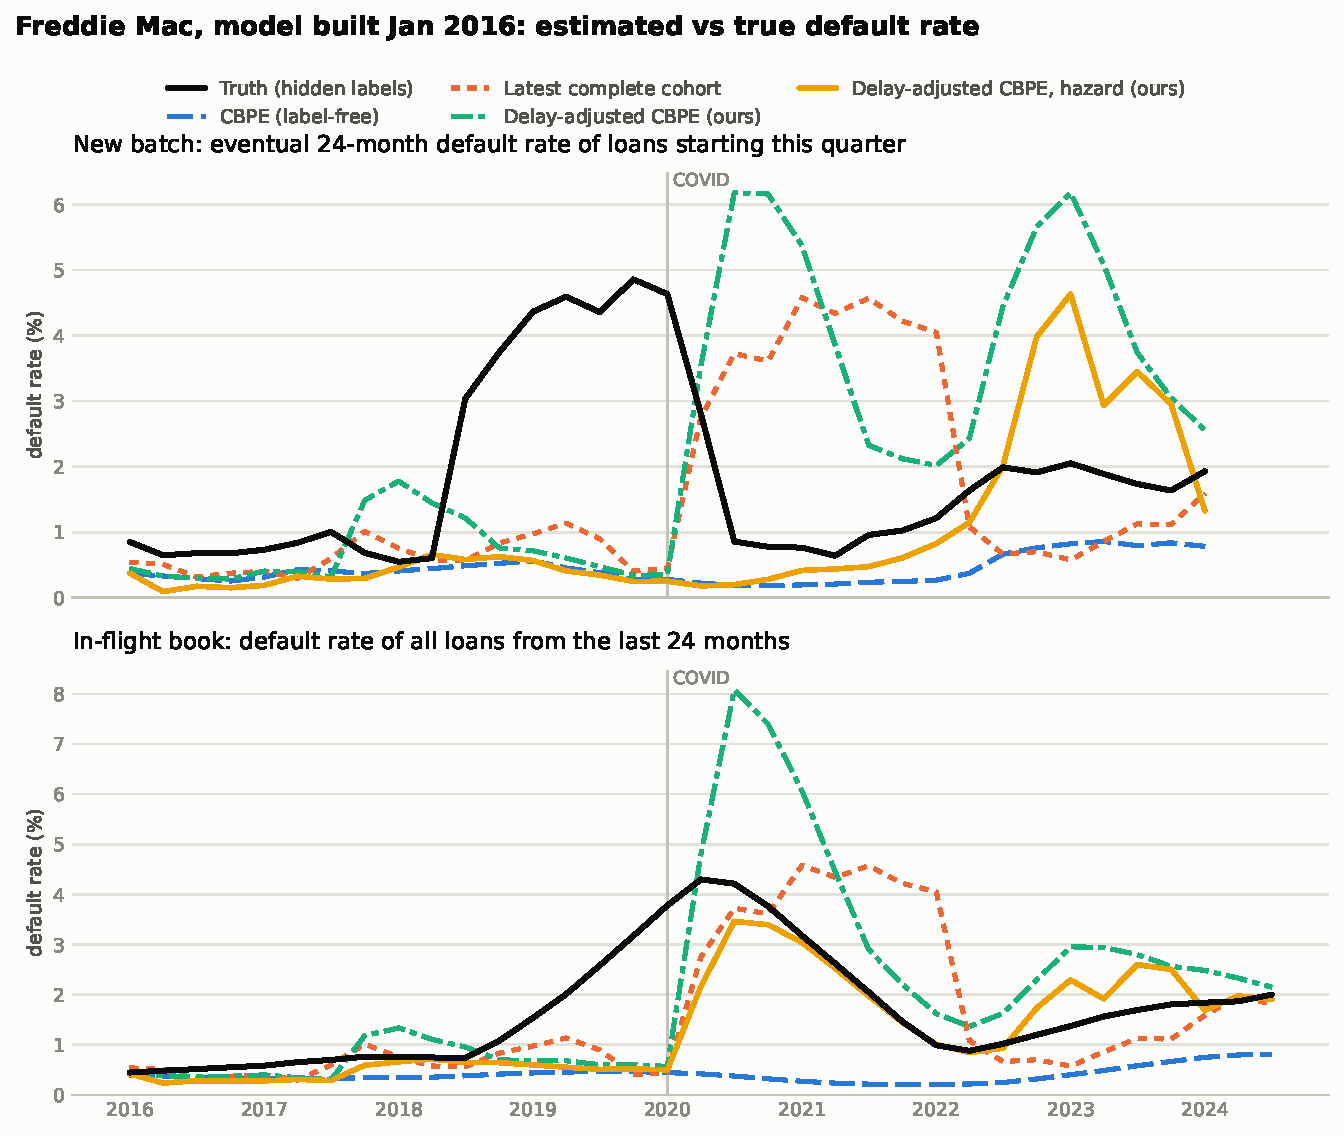
\includegraphics[width=\linewidth]{../figures/freddie_2016_default_rate.pdf}
\caption{Freddie Mac, model built January 2016 (COVID is the main shock). Top: next-batch default
rate; bottom: in-flight book.}
\label{fig:freddie16}
\end{figure}

\begin{figure}[h]
\centering
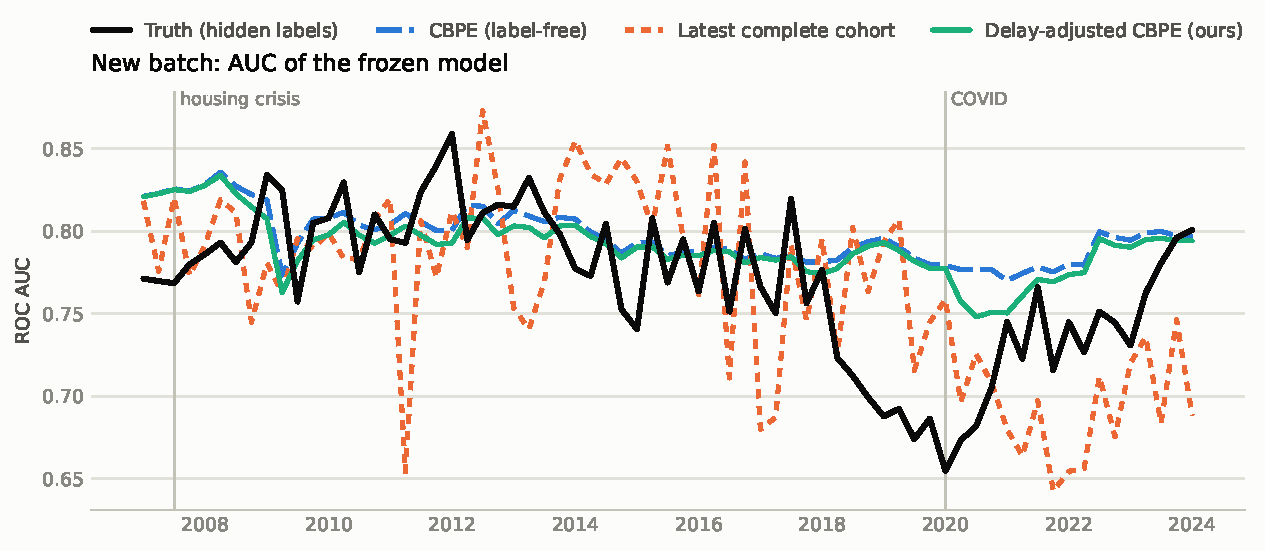
\includegraphics[width=\linewidth]{../figures/freddie_2007_auc.pdf}
\caption{Freddie Mac, model built January 2007: next-batch AUC. AUC moves less than the default
rate; label-free estimates of it stay smooth while the complete-cohort baseline is noisy.}
\label{fig:auc07}
\end{figure}

\section{Data access and licenses}\label{app:license}

ACS, BRFSS and NYC taxi records are US public-sector releases. Freddie Mac's loan-level data are free
for non-commercial research but may not be redistributed; TabReD combines Yandex data for
non-commercial research with Kaggle competition data under their rules. The repository therefore
contains no raw data: only download code, checksums, loaders and aggregated results. All sources are
de-identified public releases; the benchmark adds no personal data.

\end{document}
